% \chapter{Измерение квантовой информации Фишера в МК эксперименте ЯМР}
\chapter{Измерение информации Фишера в МК эксперименте ЯМР}
\label{chapter:quantum-fisher-information-measurement}
% (PRA-2019)
% - Расчет динамики при низкой температуре
% - Вычисление второго момента

В разделе~\ref{sec:quantum-fisher-information-mesuarement-at-high-temperature}
была обсуждена связь между вторым моментом распределения интенсивностей МК когерентностей ЯМР и квантовой информацией Фишера~\cite{Toth2014,Pezze2018}.
В частности, было показано,
что в классическом эксперименте ЯМР, когда сигнал усредняется по наблюдаемой $I_z$, в области высоких температур второй момент МК спектра соответствует нижней границе квантовой информации Фишера~\cite{Garttner2018}.
Ниже будет показано, что МК эксперимент ЯМР может быть проведен таким образом,
что связь квантовой информации Фишера и второго момента сохранится для произвольных температур.


\section{МК динамика ЯМР при низких температурах}
%\section{МК когерентности ЯМР}
\begin{figure}[H]
  \centering
  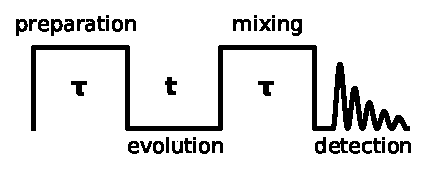
\includegraphics[width=0.5\textwidth]{mq-experiment-schema.pdf}
  \caption{Схема МК эксперимента ЯМР}
  \label{fig:mq-experiment-schema}
\end{figure}

Первоочередно рассмотрим теорию МК динамики ЯМР (см. раздел~\ref{sec:mq-nrm-experiment})
для термодинамически равновесного начального состояния системы $\rho_\mathrm{eq}$,
которое определяется выражением
%
\begin{equation}
  \label{eq:rho_eq}
  \rho_{\mathrm{eq}} = \dfrac{e^{\frac{\hbar\omega_{0}}{kT} I_z}}{Z},
\end{equation}
%
где $Z =\mathrm{Tr}\left\{e^{\frac{\hbar\omega_{0}}{kT} I_z}\right\}$ это статистическая сумма,
$\hbar$ и $k$ --- это постоянная Планка и постоянная Больцмана,
$\omega_0$ --- Ларморовская частота,
$T$ --- температура,
и $I_z$ это оператор проекции полного углового момента на ось $z$,
которая направлена вдоль сильного внешнего магнитного поля.

Для теоретического исследования МК динамики ЯМР
необходимо найти эволюционную матрицу плотности $\rho(\tau)$
на подготовительном периоде МК эксперимента ЯМР (см. раздел~\ref{sec:mq-nrm-experiment}),
решив уравнение Лиувилля~\cite{Feldman2012}
%
\begin{equation}
    \label{eq:liouvile}
    i \dfrac{d\rho(\tau)}{d \tau} =
    \left[H_\mathrm{MQ}, \rho(\tau)\right]
\end{equation}
%
с начальной матрицей плотности $\rho(0)$,
находящейся в термодинамическом равновесии,
%
\begin{equation}
    \label{eq:rho_init}
    \rho(0) = \rho_{\mathrm{eq}}
\end{equation}
%
Так как в рассматриваемом случае гамильтониан~$H_\mathrm{MQ}$
не зависит от времени,
эволюционная матрица плотности может быть выражена как
\begin{equation}
  \label{eq:rho_eval_lt}
  \rho_\mathrm{LT} (\tau) = e^{-iH_\mathrm{MQ}\tau} \rho_\mathrm{eq} e^{iH_\mathrm{MQ}\tau},
\end{equation}
В области высоких температур,
когда $b = \frac{\hbar\omega_{0}}{kT} \ll 1$,
начальную матрицу плотности $\rho_{\mathrm{eq}}$ можно разложить в ряд по $b$:
%
\begin{equation}
  \label{eq:rho_ht}
  \rho_{\mathrm{eq}} \approx \dfrac{1}{2^N} (1 + bI_z).
\end{equation}
%
В этом случае эволюционную матрицу плотности можно переписать, как
\begin{equation}\label{eq:rho_eval_ht}
  \rho_\mathrm{HT} (\tau) =  e^{-iH_\mathrm{MQ}\tau} I_z e^{iH_\mathrm{MQ}\tau},
\end{equation}

Экспериментальное исследование МК динамики ЯМР заключается в проведении
МК эксперимента ЯМР (см. раздел~\ref{sec:mq-nrm-experiment})
и последующем измерении интенсивностей МК когерентностей ЯМР.
В результате проведения всех периодов МК эксперимента ЯМР (Рис.~\ref{fig:mq-experiment-schema})
итоговый сигнал $G(\tau, \phi)$ хранится в информации о населенности\cite{Feldman1997}.
Выражение для сигнала $G(\tau, \phi)$ имеет вид
%
\begin{equation}
  \label{eq:signal}
   G(\tau, \phi)
   = \tr{
     e^{iH_\mathrm{MQ}\tau} e^{i\phi I_z} e^{-iH_\mathrm{MQ}\tau}
     \rho_\mathrm{eq}
     e^{iH_\mathrm{MQ}\tau} e^{-i\phi I_z} e^{-iH_\mathrm{MQ}\tau}
     I_z
    }.
\end{equation}
%
Перегруппировкой множителей,
выражение~(\ref{eq:signal}) может быть переписано через
 $\rho_\mathrm{LT} (\tau)$ и $\rho_\mathrm{HT} (\tau)$:
%
\begin{equation}
  \label{eq:signal-short}
  G(\tau, \phi) = \tr{
   e^{i\phi I_z} \rho_\mathrm{LT} (\tau)
   e^{-i\phi I_z} \rho_\mathrm{HT} (\tau)
  }
\end{equation}


Для получения выражений сигналов отдельных когерентностей,
перейдем к представлению матриц плотности
$\rho_\mathrm{LT} (\tau)$ и $\rho_\mathrm{HT} (\tau)$
в виде ряда
%
\begin{equation}\label{eq:rho_series}
  \rho_\mathrm{LT} (\tau) = \sum_n \rho_{LT, n}(\tau); \quad
  \rho_\mathrm{HT} (\tau) = \sum_n \rho_{HT, n}(\tau),
\end{equation}
%
где $\rho_{LT, n} (\tau)$ и  $\rho_{HT, n} (\tau)$
это вклад МК когерентности $n$-ого порядка
в матрицы плотности $\rho_\mathrm{LT} (\tau)$ и $\rho_\mathrm{HT} (\tau)$ соответственно.
Подставляя~(\ref{eq:rho_series}) в~(\ref{eq:signal}) итоговый сигнал $G(\tau, \phi)$ МК когерентностей ЯМР можно переписать как
%
\begin{equation}
    \label{eq:signal_series}
    G(\tau, \phi) = \sum\limits_n
    e^{in\phi}\mathrm{Tr} \left\{
    \rho_{LT, n}(\tau) \rho_{HT, -n} (\tau)
    \right\},
\end{equation}
%
где учтены коммутационные соотношения
%
\begin{equation}
    \left[I_z, \rho_{LT, n} (\tau) \right] = n  \rho_{LT, n} (\tau);
    \quad
    \left[I_z, \rho_{HT, n} (\tau) \right] = n  \rho_{HT, n} (\tau).
\end{equation}

Нормированные интенсивности МК когерентностей ЯМР могут быть выражены следующим образом
%
\begin{equation}
    \label{eq:coherence}
    J_n(\tau)
    = \dfrac{
       \mathrm{Tr} \left\{
        \rho_{LT, n}(\tau) \rho_{HT, -n} (\tau)
        \right\}
    }{Tr \left\{\rho_{\mathrm{eq}}I_z\right\}}.
    = \dfrac{
       \mathrm{Tr} \left\{
        \rho_{LT, n}(\tau) \rho_{HT, -n} (\tau)
        \right\}
    }{\frac N 2 \tanh \frac b 2}
\end{equation}

МК когерентности ЯМР имеют несколько свойств.
Во-первых, в момент времени  $\tau=0$
нормированная интенсивность $J_0(0)$ МК когерентности ЯМР нулевого порядка равна 1,
а остальные интенсивности равны нулю.
Во-вторых, сумма всех нормированных когерентностей равна единице.
Докажем это утверждение.
Используя выражения~(\ref{eq:rho_eq}) и~(\ref{eq:rho_eval_ht})
выразим $\rho_\mathrm{LT}(\tau)$ через $\rho_\mathrm{HT}(\tau)$.
%
\begin{equation}\label{eq:lt-through-ht}
  \rho_\mathrm{LT}(\tau) = \dfrac 1 Z
  \exp\left(be^{-iH_\mathrm{MQ}\tau} I_z e^{iH_\mathrm{MQ}\tau}\right) =
  \dfrac 1 Z e^{b\rho_\mathrm{HT}(\tau)}.
\end{equation}
%
Подставляя выражение~(\ref{eq:lt-through-ht}) в~(\ref{eq:coherence}) получаем
%
\begin{multline}
  \label{eq:sum_of_coherence}
  \sum\limits_n J_n(\tau) =
  \dfrac{\sum\limits_{n, m}\mathrm{Tr}\left\{
      \rho_{LT, n}(\tau)\rho_{HT, m}(\tau)
  \right\}}
  {\mathrm{Tr}\left\{\rho_\mathrm{eq} I_z\right\}} = \\
  \dfrac{\mathrm{Tr}\left\{
      \rho_\mathrm{LT}(\tau)\rho_\mathrm{HT}(\tau)
  \right\}}
  {\mathrm{Tr}\left\{\rho_\mathrm{eq} I_z\right\}} =
  \dfrac{\mathrm{Tr}\left\{
      \rho_\mathrm{HT}(\tau)e^{b\rho_\mathrm{HT}(\tau)}
  \right\}}
  {Z\mathrm{Tr}\left\{\rho_\mathrm{eq} I_z\right\}} = \\
  \dfrac{\frac{d}{db} \ln \mathrm{Tr}\left\{
      e^{b I_z}
  \right\}}
  {\mathrm{Tr}\left\{\rho_\mathrm{eq} I_z\right\}} =
  \dfrac{\frac 1 2 N \tanh \left( \frac b 2 \right)}
  {\frac 1 2 N \tanh \left( \frac b 2 \right)} = 1.
\end{multline}
Ур.~(\ref{eq:sum_of_coherence}) подтверждает,
что сумма МК когерентностей ЯМР сохраняется на подготовительном периоде МК эксперимента ЯМР.


\section{Приведенные МК когерентности ЯМР}
\label{sec:reduced-mq-coherences}

В предыдущем разделе было получено выражение~(\ref{eq:signal-short}) коррелятора сигнала $G(\tau, \phi)$,
которое в области высоких температур имеет вид
%
\begin{equation}
    \label{eq:otoc-ht}
    G_\mathrm{HT}(\tau, \phi) = \frac b Z\mathrm{Tr}\left\{
    e^{i \phi I_z}
    \rho_\mathrm{HT} (\tau)
    e^{-i \phi I_z}
    \rho_\mathrm{HT}(\tau)
    \right\},
\end{equation}
%
так как согласно разложению~(\ref{eq:rho_ht})
%
\begin{equation}
  \rho_\mathrm{LT} (\tau) \approx \frac 1 Z + \frac b Z \rho_\mathrm{HT}.
\end{equation}
%
Так же в разделе~\ref{sec:quantum-fisher-information-mesuarement-at-high-temperature}
было отмечено,
что связь второго момента МК спектра ЯМР и квантовой информации Фишера
обеспечивается благодаря особому виду коррелятора сигнала.
% Коррелятор должен принадлежать классу неупорядоченных по времени корреляторов ``out-of-time-ordered correlator'' (OTOC).
Выражение~(\ref{eq:otoc-ht}) для $G_\mathrm{HT}(\tau, \phi)$
в высоко температурной области
удовлетворяет этому требованию,
в отличие от выражения~(\ref{eq:signal-short}) для $G(\tau, \phi)$.
$G(\tau, \phi)$ не является неупорядоченным по времени коррелятором,
так как выражение~(\ref{eq:signal}) содержит разные матрицы $\rho_\mathrm{LT}(\tau)$ и $\rho_\mathrm{HT}(\tau)$.
Однако можно обобщить МК эксперимент ЯМР  таким образом,
чтобы привести сигнал $G(\tau, \phi)$ к нужному виду.
Для достижения такого поведения коррелятора финального сигнала МК эксперимента ЯМР
необходимо усреднить сигнал,
полученный после трех периодов %МК эксперимента ЯМР
(Рис.~\ref{fig:mq-experiment-schema}),
по начальному состоянию $\rho_\mathrm{eq}$.
Тогда коррелятор сигнала будет описываться следующим выражением
%
\begin{multline}
  \label{eq:otoc_LT}
  G_\mathrm{LT}(\tau, \phi) =
  \mathrm{Tr}\left\{
    e^{i H_{\mathrm{MQ}} \tau}
    e^{i \phi I_z}
    e^{-i H_{\mathrm{MQ}} \tau}
    \rho_{\mathrm{eq}}
    e^{i H_{\mathrm{MQ}}}
    e^{-i \phi I_z}
    e^{-i H_{\mathrm{MQ}} \tau}
    \rho_{\mathrm{eq}}
  \right\} \\ =
  \mathrm{Tr}\left\{
    e^{i \phi I_z}
    e^{-i H_\mathrm{MQ} \tau}
    \rho_\mathrm{eq}
    e^{i H_\mathrm{MQ} \tau}
    e^{-i \phi I_z}
    e^{-i H_\mathrm{MQ} \tau}
    \rho_{\mathrm{eq}}
    e^{i H_\mathrm{MQ} \tau}
  \right\} \\ =
  \mathrm{Tr}\left\{
    e^{i \phi I_z}
    \rho_\mathrm{LT} (\tau)
    e^{-i \phi I_z}
    \rho_\mathrm{LT} (\tau)
  \right\}.
\end{multline}
%
Из выражения~(\ref{eq:otoc_LT}) следует,
что $G_\mathrm{LT}(\tau, \phi)$ является неупорядоченным по времени коррелятором при произвольных температурах.
Важно отметить,
что полученный результат для начальной матрицы~(\ref{eq:rho_eq}) легко обобщить
на произвольное начальное состояние.
Связь квантовой информации Фишера и второго момента будет выполняться всегда,
если по итогу трех периодов (Рис.~\ref{fig:mq-experiment-schema}) МК экскремента ЯМР
проводить усреднение по начальному состоянию.
Это наблюдение будет играть важную роль в следующей Главе~\ref{chapter:manyparticle-entanglement-in-nanopore}
при рассмотрении МК динамики ЯМР дипольных упорядоченных состояний.

Нормированные интенсивности МК когерентностей ЯМР для сигнала $G_\mathrm{LT}(\tau, \phi)$
могут быть записаны по аналогии с~(\ref{eq:coherence}):
%
\begin{equation}\label{eq:reduced-mq-coherences}
    J_{\mathrm{LT}, n}(\tau) =
    \frac{\mathrm{Tr} \left\{
        \rho_{\mathrm{LT},n}(\tau)
        \rho_{\mathrm{LT}, -n}(\tau)
    \right\}}
    {\mathrm{Tr}\left\{\rho^2_\mathrm{eq}\right\}}.
\end{equation}
%
В этом случае нормировочный член определяется как
%
\begin{equation}\label{eq:j_lt_norm}
  \mathrm{Tr}\left\{\rho^2_\mathrm{eq}\right\} =
    \frac{2^N \cosh^N(b)}{Z^2}.
\end{equation}
Когерентности определяемые выражением~(\ref{eq:reduced-mq-coherences})
являются приведенными МК когерентностями ЯМР.
%
Используя разложение~(\ref{eq:rho_series}),
сумма интенсивностей приведенных МК когерентностей ЯМР~(\ref{eq:reduced-mq-coherences}) может быть записана как
%
\begin{multline}\label{eq:reduced-coherences-sum}
  \sum\limits_{n} J_{\mathrm{LT}, n}(\tau)
  = \dfrac{
    \tr{
      \sum\limits_{n}
      \rho_{\mathrm{LT}, n}(\tau)
      \rho_{\mathrm{LT},-n}(\tau)}
    }{
    \tr{\rho^2_\mathrm{eq} }
  }
  = \dfrac{
    \tr{
      \sum\limits_{m,n}
      \rho_{\mathrm{LT}, n}(\tau)
      \rho_{\mathrm{LT}, m}(\tau)
    }}{
    \tr{\rho^2_\mathrm{eq}}
  }
  \\
  = \dfrac{
    \tr{\rho_\mathrm{LT}^2(\tau)}
  }{
    \tr{\rho^2_\mathrm{eq}(\tau)}
  }
  = \dfrac{
    \tr{
      e^{-i H_\mathrm{MQ} \tau}
      \rho^{2}_\mathrm{eq}
      e^{i H_\mathrm{MQ} \tau}
    }
  }{
    \tr{ \rho^2_\mathrm{eq}}
  }
  = 1
\end{multline}
%
Из уравнения~(\ref{eq:reduced-coherences-sum}) можно сделать вывод, что сумма МК~когерентностей~ЯМР~сохраняется на подготовительном периоде МК~эксперимента~ЯМР~\cite{Baum1985}.


Удвоенный второй момент (дисперсия) $M_2(\tau)$ распределения интенсивностей приведенных МК когерентностей ЯМР $J_{\mathrm{LT}, n} (\tau)$
является нижней границей квантовой информации Фишера $F_{Q}$
(см. раздел~\ref{sec:quantum-fisher-information-mesuarement-at-high-temperature}):
\begin{equation}\label{eq:fisher-low-bound}
  F_{Q}(\tau) \geq 2M_2(\tau),
\end{equation}
где второй момент может быть выражен~\cite{Khitrin1997} как
%
\begin{equation}\label{eq:m2-via-coherences}
  M_2(\tau) = \sum\limits_n n^2 J_{\mathrm{LT}, n} (\tau).
\end{equation}

\section{Выводы}
В этой главе было предложено обобщение МК эксперимента ЯМР,
позволяющее измерять нижнюю границу квантовой информации Фишера
в произвольный момент времени подготовительного периода МК эксперимента ЯМР
с произвольным начальным состоянием системы.
В свою очередь квантовая информация Фишера является ключевой концепцией в квантовой теории информации
и основной мерой в квантовой метрологии.
В частности квантовая информация Фишера может выступать в качестве количественной оценки запутанных частиц в системе.
Таким образом, становится возможным исследование многочастичной запутанности в МК эксперименте ЯМР.
Более того, разработанный подход позволяет исследовать температурную зависимость многочастичной запутанности.

% При высоких температурах интенсивность МК когерентностей ЯМР может быть исследована экспериментально с помощью обычных МК экспериментов ЯМР.
Результаты полуаналитического анализа многочастичной запутанности в системе спин-несущих молекул (атомов) представлены в следующей главе~\ref{chapter:manyparticle-entanglement-in-nanopore}.